%======================================================================
\section{Closing Synthesis}
\label{sec:closing}
%======================================================================

Three observations summarize the memo.

\begin{description}
\item[The structural mapping is sound but conditional.] The pairings
core-guided $\leftrightarrow$ LBBD and IHS $\leftrightarrow$ Dantzig--Wolfe
developed in \cref{sec:part1} are correct at the level of LP duality between
primal cuts and dual columns and at the level of oracle soundness. They
break at the level of complexity (pricing is NP-complete, not polynomial),
master tractability (the practical master is integer), and primal geometry
(cores are not extreme points of a fixed polytope). Techniques whose
correctness depends only on the row--column duality should transfer;
techniques that rely on polynomial pricing or on LP master geometry should
not be expected to transfer without adaptation.

\item[The integer master is exactly where IHS leaves Dantzig--Wolfe
behind.] \Cref{sec:part2} makes this precise: IHS with an LP master is
literally column generation on the dual packing LP, while the IHS used by
real solvers solves the master as an integer program and is strictly
stronger. The difference is the integrality gap of the hitting-set
polytope---vanishing on bipartite-conflict instances (the $P_4$ trace),
positive on odd-cycle instances (the $K_3$ counterexample, where DW
terminates at $3/2$ and IHS at the true optimum $2$).

\item[Empirics confirm the qualitative predictions but reorder
priorities.] \Citet{petrova2025empirical}, surveyed in \cref{sec:part3},
find that stronger cores (maximal extraction)---the analog of
Pareto-optimal cut selection---pay off broadly: maximal cores are the
best option on $10$ of $12$ benchmark classes. On the hitting-vector axis no
option dominates: relaxed subproblems (cost-bounded, and greedy layered on
cost-bounded) win on $8$ of the $12$ classes, the exact master on the
remaining $4$, and greedy layered on the exact master never wins.
Cost-function merging, a preprocessing axis the framing of
\cref{sec:part1,sec:part2,sec:taxonomy} does not model, is the single most
impactful design choice.

\item[Open directions.] Three concrete avenues stand out. (i) The
weighted case of the equivalence: the cleanest LP encodings of core-guided
algorithms~\citep{katsirelos2023analysis} cover only unweighted instances,
and the weighted analysis is open. (ii) An LP-relaxation view of the WCSP
hitting-vector subproblem, building on the Lagrangian view of
\cref{sec:taxonomy}, would unlock the dual-stabilization and price-aware
techniques of \cref{sec:techniques} for the empirical setting of
\cref{sec:part3}. (iii) Further hybrid refinements: while basic
cross-family warm-starting behaves as predicted on the toy instances of
\cref{tab:results}, more sophisticated interleaving---e.g., dynamic switching between core-guided
and IHS phases based on progress metrics, or leveraging initial disjoint cores to heavily prune incomplete solvers like linear search \citep{berg2020core}---remains underexplored.
(iv) Extending the pricing-side program of \cref{sec:cg-gap}: the
threshold sweep (\cref{sec:price-guided}) and abstract cores
(\cref{sec:abstract-cores}) are now implemented in the prototype, and the
gap-recovery study of \cref{sec:gap-empirical} shows that aligned
aggregation recovers the full LP--IP gap of \cref{prop:nonequiv} on
odd-cycle and unit vertex-cover families while misaligned weight-class
clustering reverses the benefit. Stratified partial pricing
(\cref{sec:stratified}) remains unimplemented, and the dual-informed
clustering suggested by \cref{tab:alignment}---aggregating by the
master's price trajectories rather than by weight alone---is the natural
next experiment.
\end{description}

\paragraph{Empirical illustration.} \Cref{tab:results} reports a small
illustrative run of the techniques surveyed in \cref{sec:techniques}, produced
by \texttt{src/example.py} against the prototype \texttt{IHSSolver}
(\texttt{src/ihs.py}). Three instances are used:
\begin{itemize}
\item \textbf{$P_4$ (worked example, \cref{sec:worked}):} 4 unit soft clauses
plus 3 conflict hard clauses; LP and IP optima both $2$.
\item \textbf{$K_3$ (counterexample, \cref{sec:counter}):} 3 unit soft clauses
plus pairwise-conflict hard clauses; LP $1.5$, IP $2$.
\item \textbf{Weighted Chain:} 5 conflicting unit-clause pairs with asymmetric
weights, one hard tying clause, and one soft clause participating in multiple
cores ($10$ soft, $12$ hard total); LP and IP optima both $13$. Designed so
the stabilization techniques have non-trivial structure to act on.
\end{itemize}
Each row is one technique from \cref{sec:techniques} layered on the baseline,
plus a final \textsc{Hybrid} row enabling all of them at once. We report the
number of outer iterations, SAT-oracle calls, IP-master solves, and Pareto
refinements (additional in-search SAT calls); the returned cost and the
final LP-master value were identical across all configurations on each
instance and are reported in the caption. The warm-start seed is a
5-iteration core-guided (Fu--Malik) phase, harvested via
\texttt{coreguided.harvest\_cores}.
\Cref{tab:results} should be read as a sanity check rather than a benchmark
study: the instances are tiny and the per-iteration cost is dominated by
fixed overhead. Every configuration returned the true optimum on every instance 
(cost $2$, $2$, and $13$ respectively), with final LP-master values $2.0$, 
$1.5$, and $13.0$: on $K_3$ the LP value stays at $z^\star_{\mathrm{LP}} = 1.5$ 
while the IP master returns $z^\star = 2$, the gap predicted by \cref{prop:nonequiv}.

In the table, \textit{It} denotes outer iterations, \textit{SAT} is SAT-oracle calls, 
\textit{IP} is IP-master solves, and \textit{Pr} is Pareto refinements. Warm-start 
uses a 5-iteration Fu--Malik seed.

\begin{table}[htbp]
\centering
\small
\caption{Illustrative runs of \cref{sec:techniques} techniques on the three
toy instances shipped in \texttt{src/wcnf/}.}
\label{tab:results}
\setlength{\tabcolsep}{4.5pt}
\renewcommand{\arraystretch}{1.15}
\begin{tabular}{l cccc cccc cccc}
\toprule
& \multicolumn{4}{c}{\textbf{$P_4$ (worked)}}
& \multicolumn{4}{c}{\textbf{$K_3$ (counter)}}
& \multicolumn{4}{c}{\textbf{Weighted Chain}} \\
\cmidrule(lr){2-5} \cmidrule(lr){6-9} \cmidrule(lr){10-13}
\textbf{Config.}
& It & SAT & IP & Pr
& It & SAT & IP & Pr
& It & SAT & IP & Pr \\
\midrule
Plain IHS (baseline)         & 3 & 3 & 3 & 0  & 4 & 4 & 4 & 0  & 7 & 7  & 7 & 0 \\
+ Warm-start (Fu--Malik seed)& 1 & 1 & 1 & 0  & 2 & 2 & 2 & 0  & 2 & 2  & 2 & 0 \\
+ Pareto core selection      & 3 & 4 & 3 & 0  & 4 & 6 & 4 & 0  & 7 & 19 & 7 & 0 \\
+ Box penalty ($\alpha_0{=}1$, $\rho{=}0.5$)
                              & 3 & 3 & 3 & 0  & 4 & 4 & 4 & 0  & 7 & 7  & 7 & 0 \\
+ In-out separation ($\lambda{=}0.5$)
                              & 3 & 5 & 3 & 0  & 4 & 7 & 4 & 0  & 7 & 13 & 7 & 0 \\
+ Price-aware ordering       & 3 & 3 & 3 & 0  & 4 & 4 & 4 & 0  & 7 & 7  & 7 & 0 \\
\textsc{Hybrid} (all)        & 1 & 1 & 1 & 0  & 2 & 4 & 2 & 0  & 2 & 8  & 2 & 0 \\
\bottomrule
\end{tabular}
\end{table}

\paragraph{Reading the table.} Three observations, all weak by design (the
instances are too small for anything stronger):
\begin{enumerate}
\item \textbf{Correctness.} All configurations return $z^\star$ on all three
instances. In particular, on $K_3$ the IHS-IP master correctly returns
$z^\star = 2$ even though the LP master value remains $1.5$---the gap predicted
by \cref{prop:nonequiv}.

\item \textbf{Warm-start dominates iteration count.} On each instance, warm
starting from a 5-step core-guided phase collapses the outer loop to
$1$--$2$ iterations: the seeded master already contains enough cores that the
first SAT call either certifies optimality immediately ($P_4$) or needs one
more cut ($K_3$, Weighted Chain). This is the cleanest empirical signal in the
table.

\item \textbf{Stabilization techniques are inactive at this scale.} The
box-penalty stabilizer and price-aware ordering produce numerically identical
runs to the baseline, and
in-out separation and Pareto selection only add SAT calls without changing the
iteration count or the cores discovered. This is consistent with their
intended regime---late-phase tailing-off on degenerate masters---which the
toy instances do not exhibit. The \textsc{Hybrid} row is essentially
warm-start with additional SAT overhead from in-out and Pareto.
\end{enumerate}

A meaningful evaluation of the stabilization axis requires instances large
enough to exhibit master degeneracy and dual oscillation. To this end, 
parameterized benchmarks have been implemented and tested for structured families 
including Vertex Cover, Weighted Set Cover, and Weighted Max-3SAT. 
As shown in \cref{fig:benchmarks,fig:additional_benchmarks}, 
an ablation study reveals surprising dynamics between the transferred techniques. 

On the Vertex Cover and Weighted Set Cover instances, the \emph{Multi-core extraction} 
feature emerges as the overwhelmingly dominant factor, independently reducing the number 
of outer iterations and overall runtime by more than a factor of three compared to the 
baseline IHS. This completely aligns with the foundational Implicit Hitting Set literature 
(\citealp{davies2011solving, davies2013exploiting}), which established that extracting multiple 
disjoint cores per iteration is crucial for preventing the IP master from stalling. Interestingly, the \textsc{Hybrid} configuration---which enables all stabilization, 
warm-starting, and pricing features simultaneously---actually performs \emph{worse} 
than the bare Multi-core extension on these problems. This points to negative interference: the 
aggressive dual-stabilization (Wentges) and modified core structures (Pareto selection) 
likely restrict the SAT oracle's ability to efficiently harvest large numbers of 
disjoint cores in a single pass. This suggests that while individual BnP techniques 
are potent, their interaction in the MaxSAT context requires careful, dynamic tuning 
rather than static composition.

Conversely, the Weighted Max-3SAT instances (\cref{fig:additional_benchmarks}, bottom row) 
highlight an important boundary condition: pushing the clause-to-variable ratio to $C=6V$ 
places the instances firmly in the unsatisfiable, exponentially difficult regime. Here, 
unlike Set Cover, the baseline solver rapidly hits an exponential wall, while the 
warm-started and multi-core configurations manage to stave off the explosion slightly 
longer. This confirms that while the core-extraction framework transfers universally,
its relative advantage depends heavily on the constraint geometry of the problem.

The same qualitative picture extends to three structured scheduling
families (\cref{fig:scheduling_1,fig:scheduling_2,fig:scheduling_3}):
task--machine allocation (generalized assignment), airport gate allocation
with conflicts, and employee shift scheduling. In all three, Multi-core
extraction again dominates the other techniques, converging in a fraction
of the baseline's iterations across every problem size tested.

\begin{figure}[htbp]
\centering
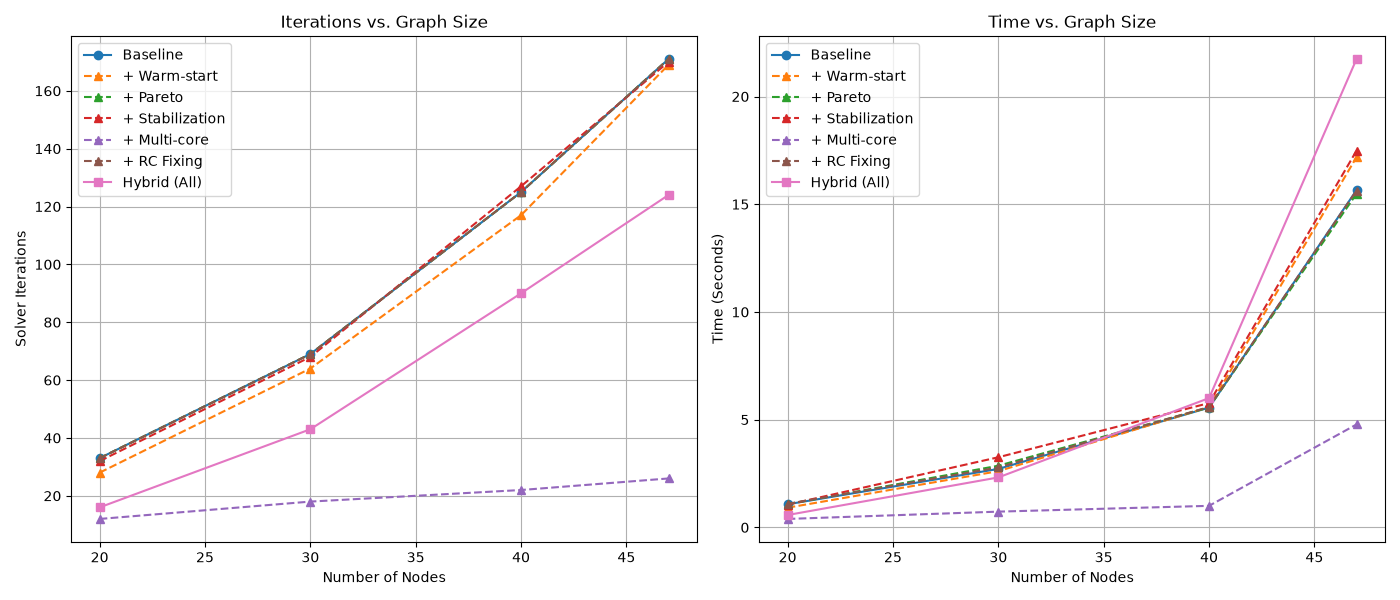
\includegraphics[width=\textwidth]{benchmark_plot.png}
\caption{Ablation study of iterations and execution time across parameterized graph sizes ($N \in \{15, 25, 35, 45\}$) for the Vertex Cover problem. The Multi-core configuration dominates all others, while the Hybrid composition exhibits negative interference.}
\label{fig:benchmarks}
\end{figure}

\begin{figure}[htbp]
\centering
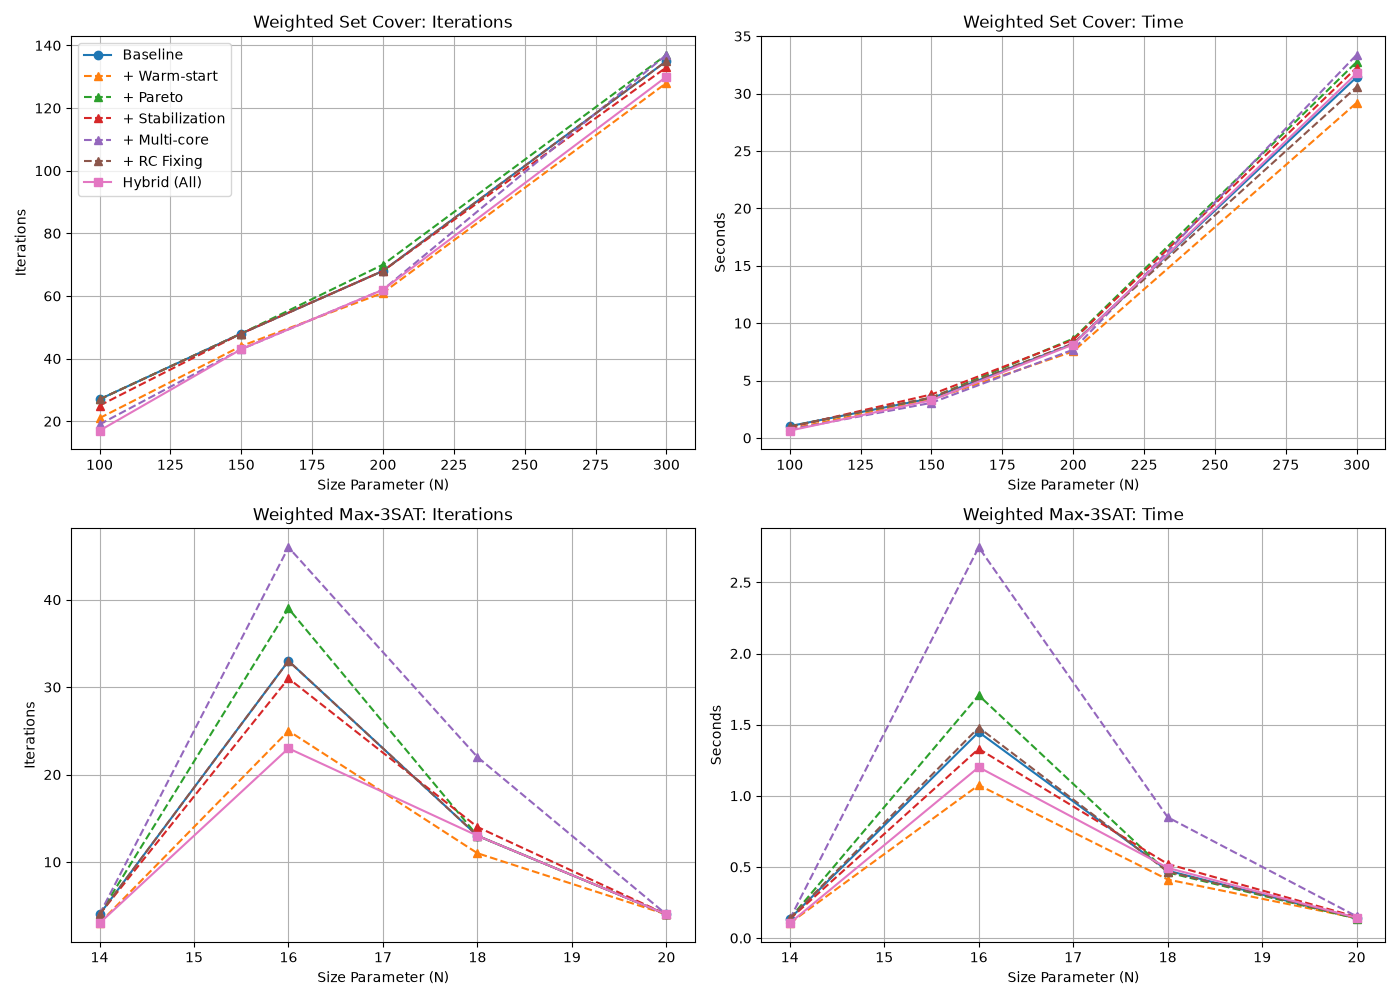
\includegraphics[width=\textwidth]{additional_plot.png}
\caption{Ablation study for Weighted Set Cover (top) and Weighted Max-3SAT (bottom). The Set Cover results mirror the Vertex Cover dynamics, while Max-3SAT at $C=6V$ pushes the solver into exponential difficulty.}
\label{fig:additional_benchmarks}
\end{figure}

\begin{figure}[htbp]
\centering
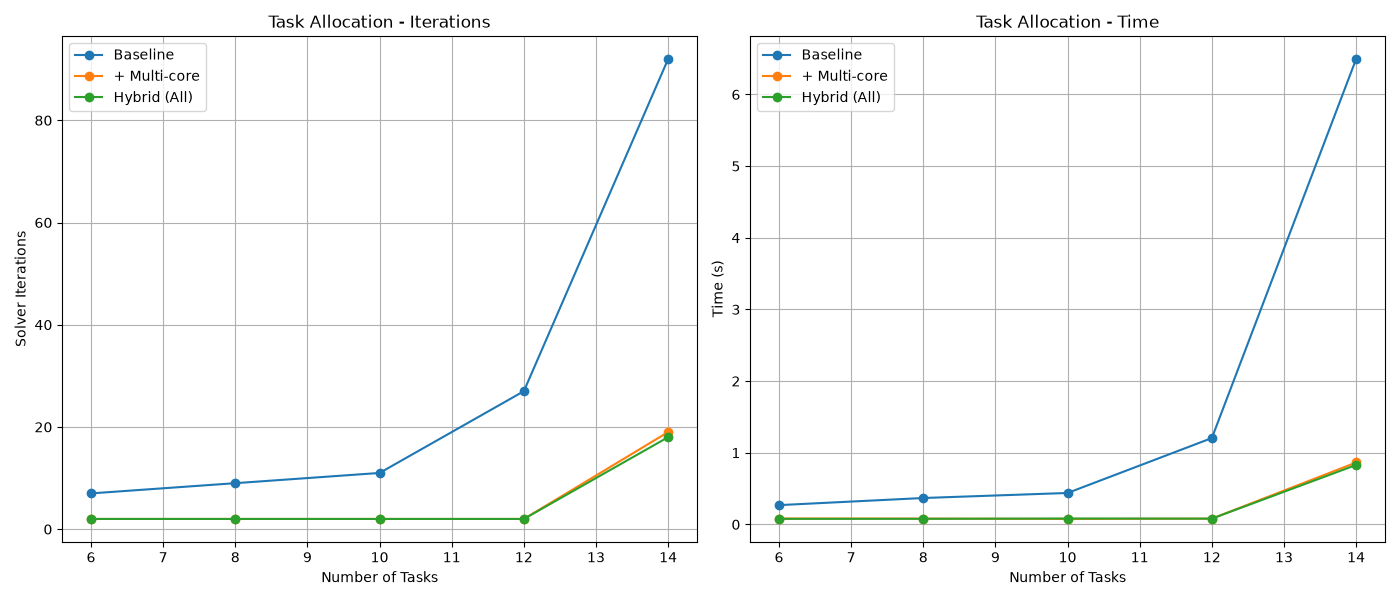
\includegraphics[width=\textwidth]{scheduling_plot_1.png}
\caption{Ablation study for Task-Machine Allocation (Generalized Assignment). Demonstrates extremely fast convergence with the Multi-core technique.}
\label{fig:scheduling_1}
\end{figure}

\begin{figure}[htbp]
\centering
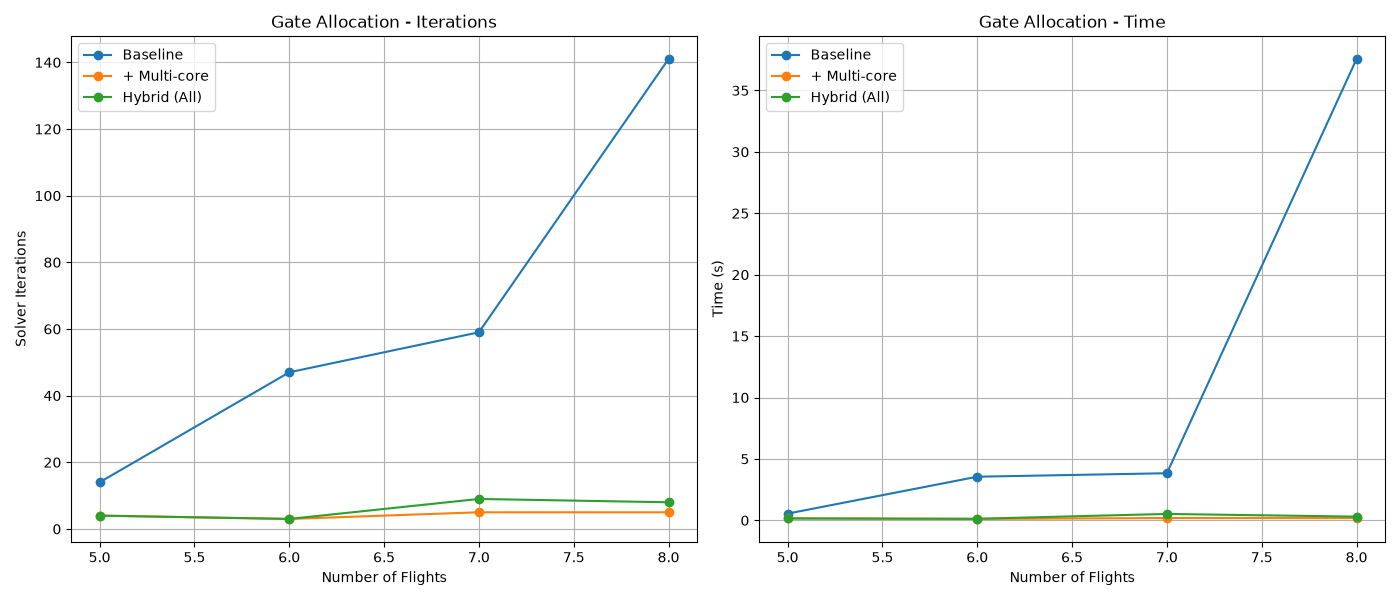
\includegraphics[width=\textwidth]{scheduling_plot_2.png}
\caption{Ablation study for Airport Gate Allocation with Conflicts. Highlights the heavy iteration requirements of the baseline and the massive advantage of Multi-core extraction.}
\label{fig:scheduling_2}
\end{figure}

\begin{figure}[htbp]
\centering
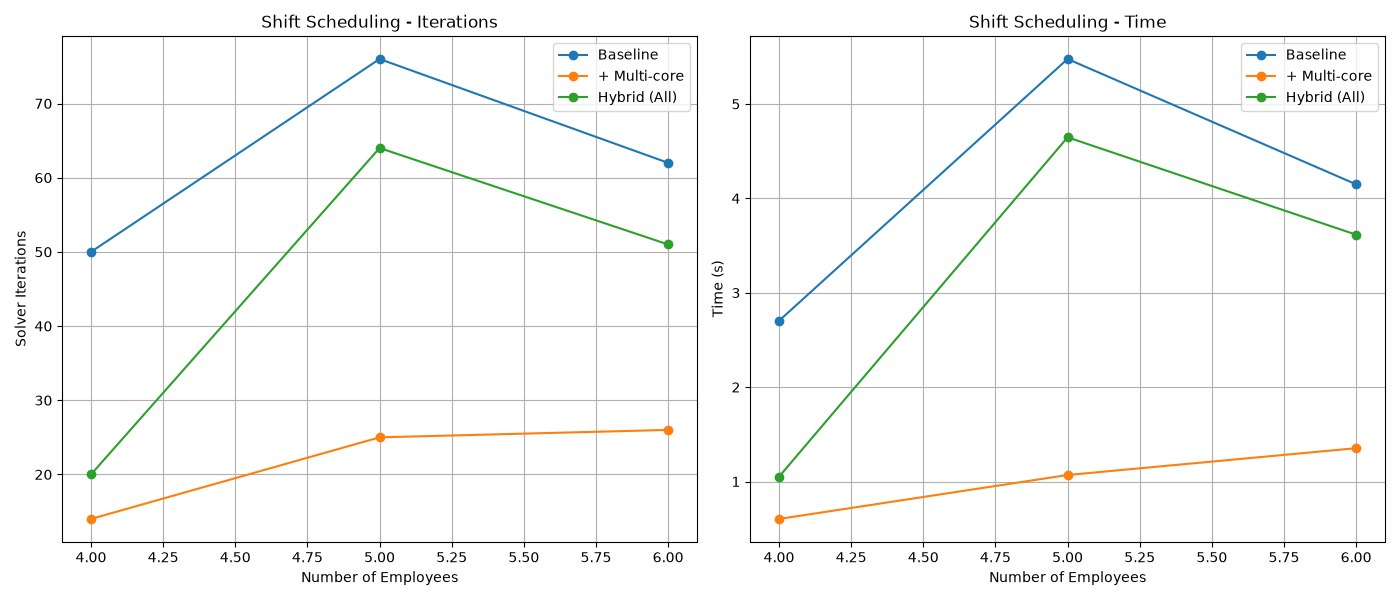
\includegraphics[width=\textwidth]{scheduling_plot_3.png}
\caption{Ablation study for Employee Shift Scheduling. Shows the robust improvement over the baseline by the Multi-core technique across various employee team sizes.}
\label{fig:scheduling_3}
\end{figure}
